% Generated from the public primitive catalog. Original Atlas drawing; Apache-2.0.
% Target: cmac-aes-192; view: overview
\documentclass[border=9pt]{standalone}
% Original Atlas figure theme. Apache-2.0; see the repository LICENSE.
\usepackage[T1]{fontenc}
\usepackage{lmodern}
\usepackage{amsmath,amssymb}
\usepackage{tikz}
\usetikzlibrary{arrows.meta,positioning,calc,fit,backgrounds,decorations.pathreplacing,matrix}
\definecolor{atlasInk}{HTML}{172235}
\definecolor{atlasTeal}{HTML}{0D7B7D}
\definecolor{atlasMuted}{HTML}{637278}
\definecolor{atlasFill}{HTML}{EAF4F2}
\definecolor{atlasLine}{HTML}{B6C8C7}
\tikzset{
  every picture/.style={line width=.65pt,draw=atlasInk,>=Latex},
  every node/.style={text=atlasInk,font=\sffamily\small},
  box/.style={draw,rounded corners=1.5pt,minimum height=.9cm,minimum width=1.6cm,align=center,inner sep=6pt,fill=white},
  accent/.style={box,draw=atlasTeal,fill=atlasFill},
  wire/.style={->,line width=.7pt},
  keywire/.style={wire,draw=atlasTeal,dashed},
  xor/.style={draw,circle,fill=white,inner sep=0pt,minimum size=.38cm},
  add/.style={draw,rectangle,fill=white,inner sep=0pt,minimum size=.38cm},
  note/.style={font=\sffamily\scriptsize,text=atlasMuted,align=center},
  phase/.style={font=\sffamily\small\bfseries,text=atlasTeal},
  group/.style={draw=atlasLine,dashed,rounded corners=2pt,inner sep=8pt}
}
\newcommand{\rotl}{\mathbin{\lll}}
\newcommand{\rotr}{\mathbin{\ggg}}
\newcommand{\kx}{\operatorname{Keccak}\!\text{-}\!f[1600]}

\newcommand{\AtlasKeyBits}{192}
\newcommand{\AtlasKeyWords}{6}
\newcommand{\AtlasRounds}{N_r}
\newcommand{\AtlasPriorRounds}{N_r-1}
\newcommand{\AtlasRoundKeys}{N_r+1}
\newcommand{\AtlasDoubleRounds}{N_r/2}
\newcommand{\AtlasSixRoundGroups}{N_r/6}
\newcommand{\AtlasFLGroups}{N_r/6-1}
\newcommand{\AtlasRoundStart}{24-n}
\newcommand{\AtlasBlockBits}{128}
\newcommand{\AtlasOutputBits}{d}
\newcommand{\AtlasStateBits}{8w}
\newcommand{\AtlasNonceBits}{v}
\newcommand{\AtlasCounterBits}{q}
\newcommand{\AtlasStreamBlockBits}{b}
\newcommand{\AtlasRate}{r}
\newcommand{\AtlasCapacity}{c}
\newcommand{\AtlasSteps}{N}
\newcommand{\AtlasLastStep}{N-1}
\newcommand{\AtlasWordBits}{w}
\newcommand{\AtlasHashWords}{h}
\newcommand{\AtlasFeedForward}{\boxplus}
\newcommand{\AtlasByteOrder}{big-endian}
\newcommand{\AtlasDomain}{01}
\newif\ifAtlasXof
\AtlasXoffalse
\begin{document}
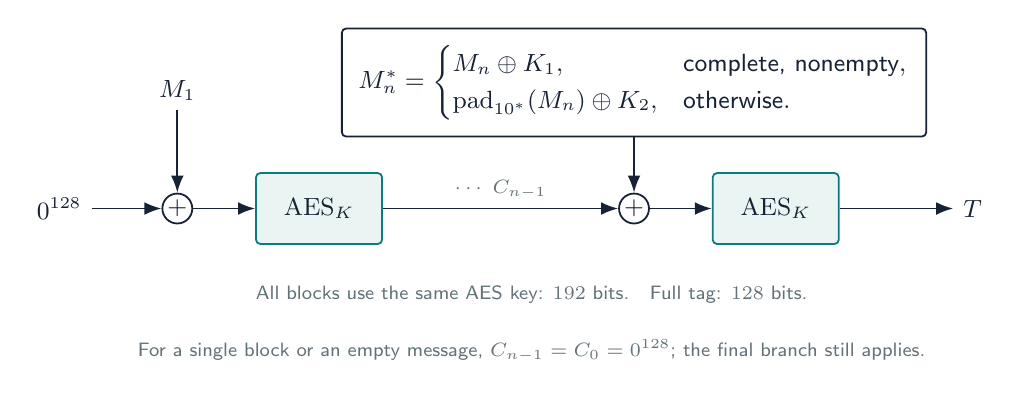
\begin{tikzpicture}
  \node (iv) at (0,0) {$0^{128}$};
  \node[xor] (x1) at (1.5,0) {$+$}; \node[accent] (e1) at (3.3,0) {$\mathrm{AES}_K$};
  \node[xor] (xn) at (7.3,0) {$+$}; \node[accent] (en) at (9.1,0) {$\mathrm{AES}_K$};
  \node (tag) at (11.6,0) {$T$};
  \draw[wire] (iv) -- (x1); \draw[wire] (x1) -- (e1);
  \draw[wire] (e1) -- node[above,note] {$\cdots\ C_{n-1}$} (xn); \draw[wire] (xn) -- (en); \draw[wire] (en) -- (tag);
  \node (m1) at (1.5,1.5) {$M_1$}; \draw[wire] (m1) -- (x1);
  \node[box,minimum width=5.5cm] (last) at (7.3,1.6) {$M_n^*=\begin{cases}M_n\oplus K_1,&\text{complete, nonempty},\\ \operatorname{pad}_{10^*}(M_n)\oplus K_2,&\text{otherwise}.\end{cases}$};
  \draw[wire] (last) -- (xn);
  \node[note] at (6,-1.1) {All blocks use the same AES key: $\AtlasKeyBits$ bits.\quad Full tag: $128$ bits.};
  \node[note] at (6,-1.8) {For a single block or an empty message, $C_{n-1}=C_0=0^{128}$; the final branch still applies.};
\end{tikzpicture}

\end{document}
